\chapter*{Tarefa - 3}

\section*{Enunciado}

\begin{figure}[h!]
\centering
\caption{Enunciado da Tarefa 3.}
\centering
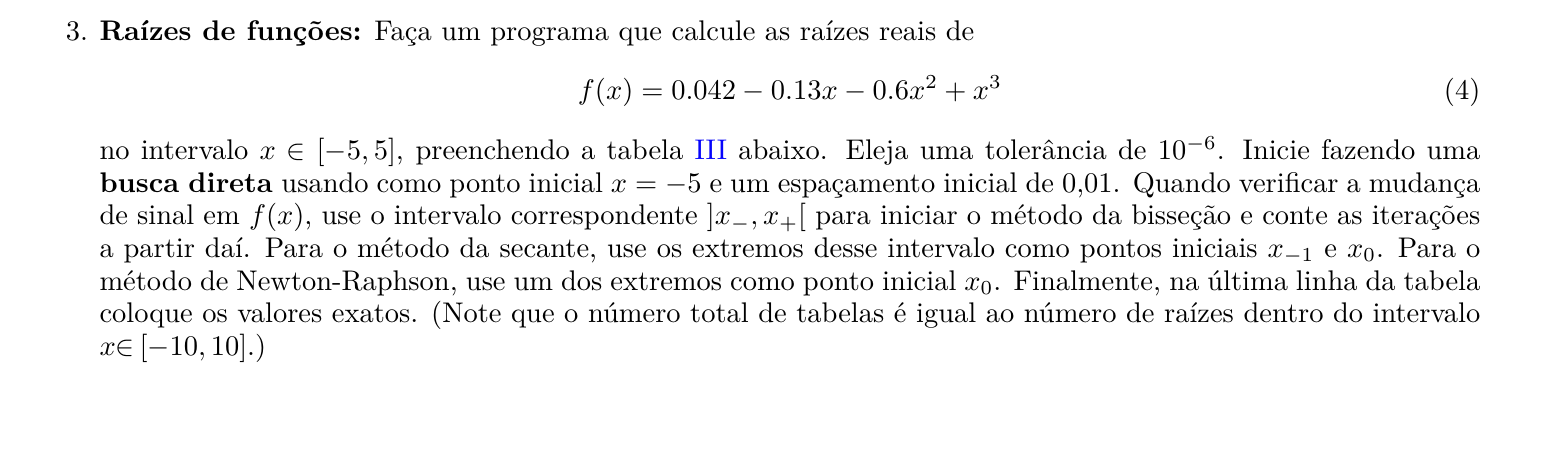
\includegraphics[width=16cm]{images/tarefa-3/enunciado-tarefa-3.png}
\caption*{Fonte: Compilado pelo Autor.}
\label{fig:tarefa 3 - Enunciado}
\end{figure}

\begin{figure}[h!]
\centering
\caption{Tarefa enunciado da Tarefa 3.}
\centering
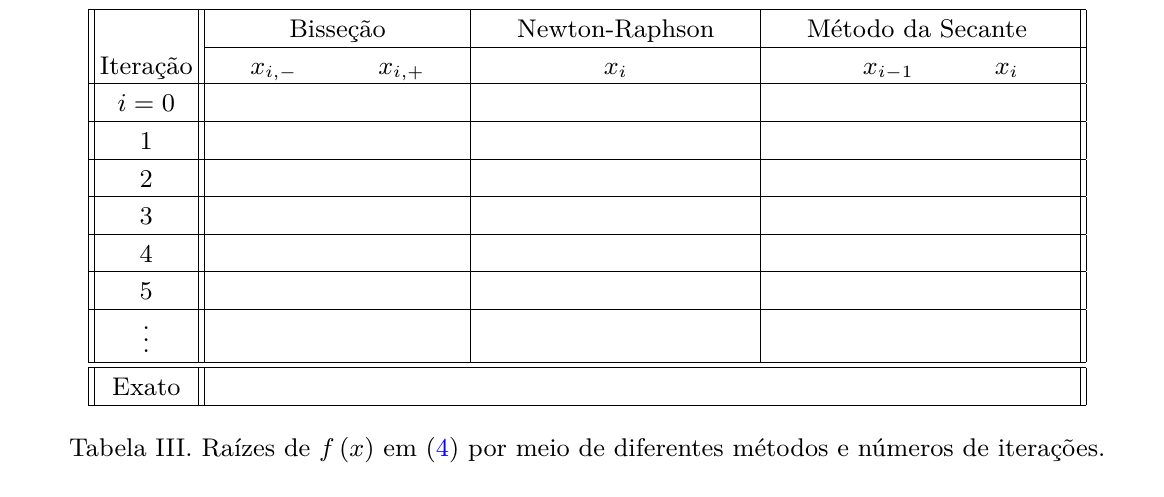
\includegraphics[width=16cm]{images/tarefa-3/tabela-enunciado-tarefa-3.png}
\caption*{Fonte: Compilado pelo Autor.}
\label{fig:tarefa 3 - Tabela Enunciado}
\end{figure}

\section*{Código}

\section*{Descrição do código}

O programa \texttt{main} tem como objetivo determinar numericamente as raízes da função

\begin{equation}
	f(x) = 0.042 - 0.13x - 0.6x^2 + x^3
\end{equation}

\noindent
utilizando três métodos iterativos de busca de raízes: 
\textbf{bisseção}, \textbf{Newton-Raphson} e \textbf{secante}.  
Cada método é implementado em uma função separada, e seus resultados são exibidos na tela e gravados em arquivos distintos.  
O código também avalia a convergência dos métodos a partir do número de iterações até atingir a tolerância estabelecida.

\bigskip
No início do programa, é utilizada a diretiva:

\vspace*{1\baselineskip}
\begin{lstlisting}
implicit real*8 (a-h,o-z)
\end{lstlisting}

\noindent
que define todas as variáveis cujos nomes começam com as letras 
de \textbf{a} a \textbf{h} e \textbf{o} a \textbf{z} como números reais 
de dupla precisão. Em seguida, são definidas as constantes principais:

\vspace*{1\baselineskip}
\begin{lstlisting}
a = 0.5d0
b = 5d0
tol = 1d-6
\end{lstlisting}

\noindent
onde $a$ e $b$ representam os limites iniciais do intervalo de busca e 
\texttt{tol} define a tolerância do erro desejado.

\bigskip
O programa principal chama as três funções numéricas responsáveis por 
calcular as raízes da função \texttt{f(x)}:

\vspace*{1\baselineskip}
\begin{lstlisting}
write(*,1) 'Bisseção: ', bissec(a,b,tol)
write(*,1) 'Newton-Raphson: ', raphson(a,tol)
write(*,1) 'Secante: ', secante(a,tol)
\end{lstlisting}

\noindent
Cada chamada executa o método correspondente e imprime o resultado com o formato:

\vspace*{1\baselineskip}
\begin{lstlisting}
1 format(A15,F14.12)
\end{lstlisting}

\noindent
permitindo visualizar o valor da raiz com 12 casas decimais de precisão.

\subsection*{Funções auxiliares}

As funções implementam tanto a função principal e sua derivada, 
quanto os três métodos iterativos de determinação de raízes.

\begin{enumerate}
	\item \textbf{Função \texttt{f(x)}} \\
	Define a função cúbica a ser analisada:
	\begin{equation}
		f(x) = 0.042 - 0.13x - 0.6x^2 + x^3
	\end{equation}

	\item \textbf{Função \texttt{df(x)}} \\
	Define a derivada de $f(x)$, necessária para o método de Newton-Raphson:
	\begin{equation}
		f'(x) = -0.13 - 1.2x + 3x^2
	\end{equation}

	\item \textbf{Função \texttt{bissec(a,b,tol)}} — Método da Bisseção \\
	O método da bisseção busca um intervalo $[a,b]$ onde há troca de sinal em $f(x)$.  
	Inicialmente, o código realiza uma varredura incremental com passo \texttt{stp = 0.01}, até encontrar um subintervalo onde $f(a)f(a+stp) < 0$.  
	Em seguida, aplica-se o procedimento iterativo:
	\begin{equation}
		c = \frac{a + b}{2}, \qquad
		\text{se } f(a)f(c) < 0, \; b = c, \; \text{senão } a = c
	\end{equation}
	até que $|b - a| < \texttt{tol}$.  
	Os valores intermediários de $c$ são gravados no arquivo:
	\vspace*{1\baselineskip}
	\begin{lstlisting}
	open(unit=13,file='saida-1-12694394.txt')
	\end{lstlisting}
	com o formato:
	\vspace*{1\baselineskip}
	\begin{lstlisting}
	14 format(I3,F16.12)
	\end{lstlisting}

	\item \textbf{Função \texttt{raphson(x,tol)}} — Método de Newton-Raphson \\
	Este método utiliza a fórmula iterativa:
	\begin{equation}
		x_{k+1} = x_k - \frac{f(x_k)}{f'(x_k)}
	\end{equation}
	As iterações continuam enquanto $|f(x)/f'(x)| > \texttt{tol}$.  
	A cada passo, o par $(\texttt{iter},x_k)$ é escrito no arquivo:
	\vspace*{1\baselineskip}
	\begin{lstlisting}
	open(unit=15,file='saida-2-12694394.txt')
	\end{lstlisting}
	usando o formato:
	\vspace*{1\baselineskip}
	\begin{lstlisting}
	16 format(I3,F16.12)
	\end{lstlisting}

	\item \textbf{Função \texttt{secante(x,tol)}} — Método da Secante \\
	Este método aproxima a derivada por diferenças finitas entre dois pontos consecutivos, conforme:
	\begin{equation}
		x_{k+1} = x_k - f(x_k)\frac{x_k - x_{k-1}}{f(x_k) - f(x_{k-1})}
	\end{equation}
	Sendo \texttt{stp = 0.01} o deslocamento inicial.  
	O processo é repetido até que $|x_{k+1} - x_k| < \texttt{tol}$.  
	Os valores iterativos são gravados em:
	\vspace*{1\baselineskip}
	\begin{lstlisting}
	open(unit=17,file='saida-3-12694394.txt')
	\end{lstlisting}
	com o formato:
	\vspace*{1\baselineskip}
	\begin{lstlisting}
	18 format(I3,F16.12)
	\end{lstlisting}
\end{enumerate}

\noindent
Assim, o programa permite determinar numericamente as raízes de uma função cúbica, 
comparando a eficiência e a convergência dos três métodos clássicos de busca de raízes: 
bisseção, Newton-Raphson e secante.  
Cada método gera um arquivo contendo as iterações realizadas, permitindo visualizar o comportamento da convergência.


\section*{Resultados}
As tabelas abaixo apresentam os resultados obtidos para as três raízes da função $f(x) = 0.042 - 0.13x - 0.6x^2 + x^3$ utilizando os métodos de Bissecção, Newton-Raphson e Secante.

\begin{table}[H]
\centering
\caption{Raízes de $f(x)$ por meio de diferentes métodos e números de iterações.}
\label{table:tarefa-3-resultados}
\begin{NiceTabular}{c|c|c|c}[hvlines, columns-width=2.8cm]
\CodeBefore
    \rowcolor{cyan}{1}
    \rowcolors{2}{cyan!25}{cyan!15}
\Body
    \RowStyle[color=white, bold]{}
    Iteração & \textbf{Bissecção} & \textbf{Newton} & \textbf{Secante} \\

    0  & -0.29500000 & -0.3000000 & -0.3000000 \\
    1  & -0.29750000 &            &      \\
    2  & -0.29875000 &            &      \\
    3  & -0.29937500 &            &      \\
    4  & -0.29968750 &            &      \\
    5  & -0.29984375 &            &      \\
    6  & -0.29992188 &            &      \\
    7  & -0.29996094 &            &      \\
    8  & -0.29998047 &            &      \\
    9  & -0.29999023 &            &      \\
    10 & -0.29999512 &            &      \\
    11 & -0.29999756 &            &      \\
    12 & -0.29999878 &            &      \\
    13 & -0.29999939 &            &      \\

    \hline
    \textbf{Raiz Aproximada} & \multicolumn{3}{c}{-0.3} \\
\end{NiceTabular}

\caption*{Fonte: Compilado pelo Autor.}
\end{table}

\begin{table}[H]
\centering
\caption{Raízes de $f(x)$ por meio de diferentes métodos e números de iterações.}
\label{table:tarefa-3-resultados-2}
\begin{NiceTabular}{c|c|c|c}[hvlines, columns-width=2.8cm]
\CodeBefore
    \rowcolor{cyan}{1}
    \rowcolors{2}{cyan!25}{cyan!15}
\Body
    \RowStyle[color=white, bold]{}
    Iteração & \textbf{Bissecção} & \textbf{Newton} & \textbf{Secante} \\

    0  & 0.1950000000& 0.19999938960& 0.200000000 \\
    1  & 0.1975000000&              &             \\
    2  & 0.1987500000&              &             \\
    3  & 0.1993750000&              &             \\
    4  & 0.1996875000&              &             \\
    5  & 0.1998437500&              &             \\
    6  & 0.1999218750&              &             \\
    7  & 0.1999609375&              &             \\
    8  & 0.1999804688&              &             \\
    9  & 0.1999902344&              &             \\
    10 & 0.1999951172&              &             \\
    11 & 0.1999975586&              &             \\
    12 & 0.1999987793&              &             \\
    13 & 0.1999993896&              &             \\

    \hline
    \textbf{Raiz Aproximada} & \multicolumn{3}{c}{0.2} \\
\end{NiceTabular}

\caption*{Fonte: Compilado pelo Autor.}
\end{table}

\begin{table}[H]
\centering
\caption{Raízes de $f(x)$ por meio de diferentes métodos e números de iterações.}
\label{table:tarefa-3-resultados-3}
\begin{NiceTabular}{c|c|c|c}[hvlines, columns-width=2.8cm]
\CodeBefore
    \rowcolor{cyan}{1}
    \rowcolors{2}{cyan!25}{cyan!15}
\Body
    \RowStyle[color=white, bold]{}
    Iteração & \textbf{Bissecção} & \textbf{Newton} & \textbf{Secante} \\

    0  & 0.695000000000 & 0.69999939 & 0.70000000 \\
    1  & 0.697500000000 &            &             \\
    2  & 0.698750000000 &            &             \\
    3  & 0.699375000000 &            &             \\
    4  & 0.699687500000 &            &             \\
    5  & 0.699843750000 &            &             \\
    6  & 0.699921875000 &            &             \\
    7  & 0.699960937500 &            &             \\
    8  & 0.699980468750 &            &             \\
    9  & 0.699990234375 &            &             \\
    10 & 0.699995117188 &            &             \\
    11 & 0.699997558594 &            &             \\
    12 & 0.699998779297 &            &             \\
    13 & 0.699999389648 &            &             \\

    \hline
    \textbf{Raiz Aproximada} & \multicolumn{3}{c}{0.7} \\
\end{NiceTabular}

\caption*{Fonte: Compilado pelo Autor.}
\end{table}

\begin{figure}[H]
\centering
\caption{Gráfico da função $f$.}
\centering
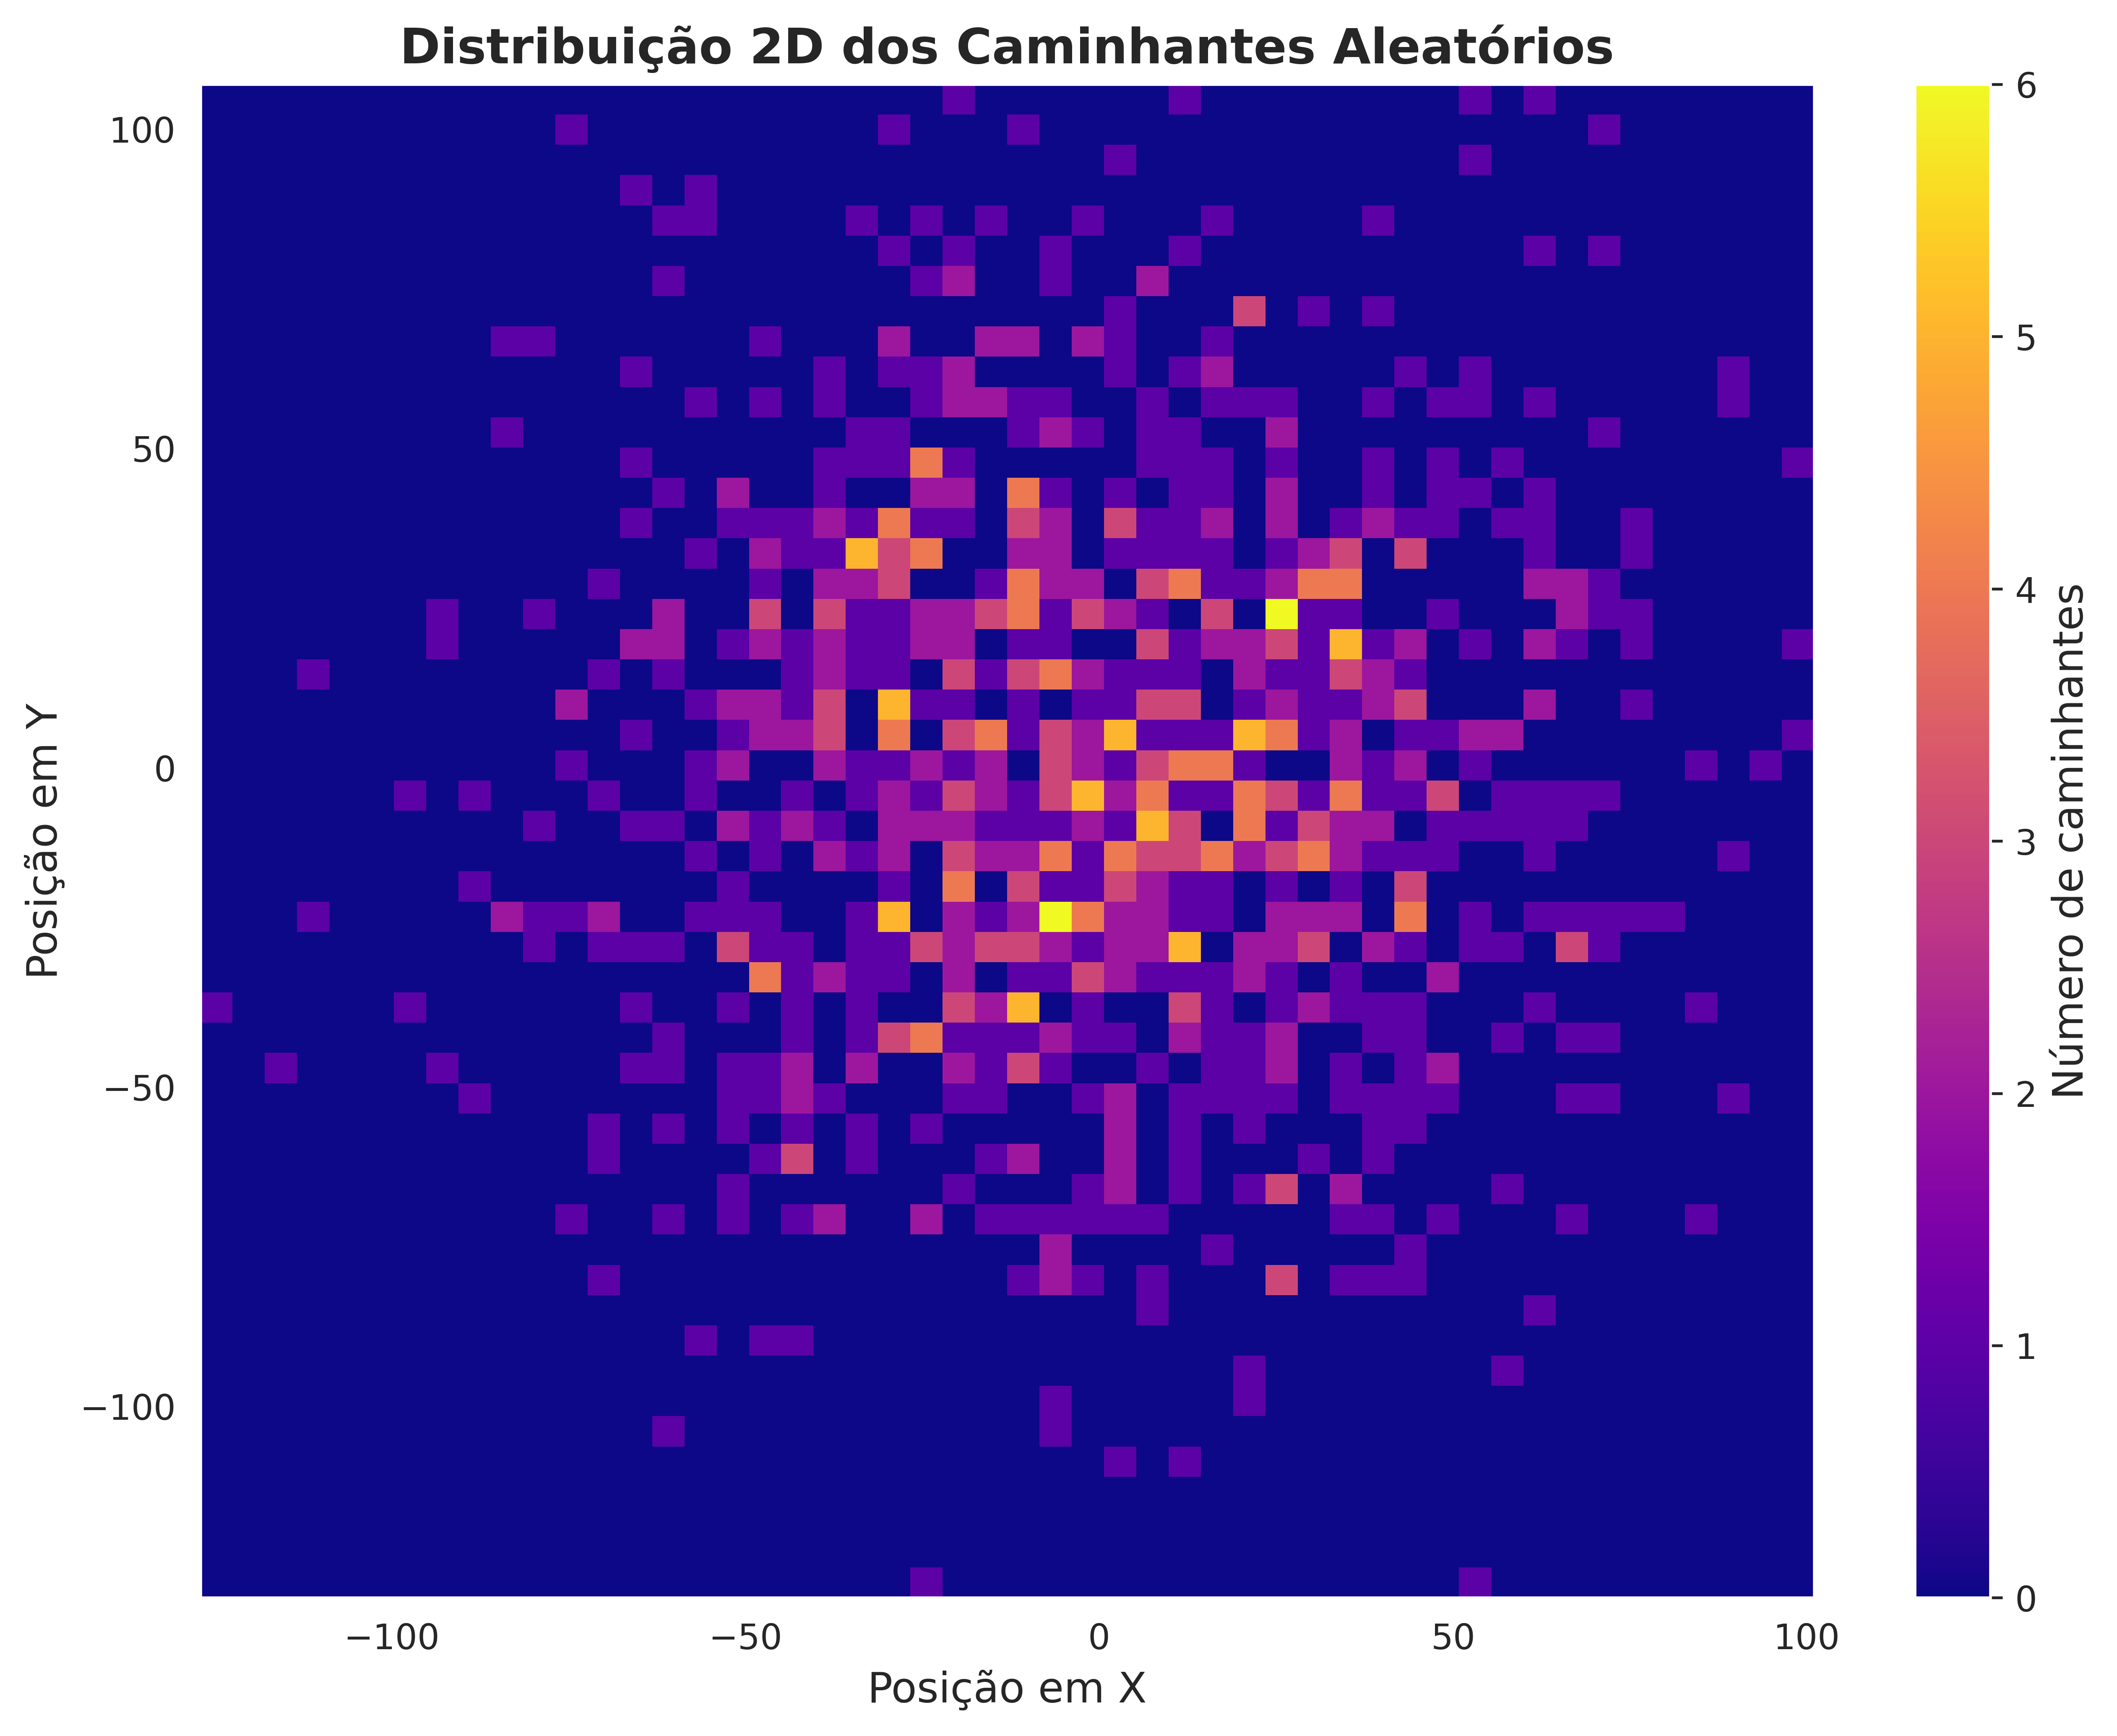
\includegraphics[width=16cm]{images/tarefa-3/tarefa-3-graf-1.png}
\caption*{Fonte: Compilado pelo Autor.}
\label{fig:tarefa 3 - Gráfico 1}
\end{figure}

\begin{figure}[H]
\centering
\caption{Gráfico da função $f$.}
\centering
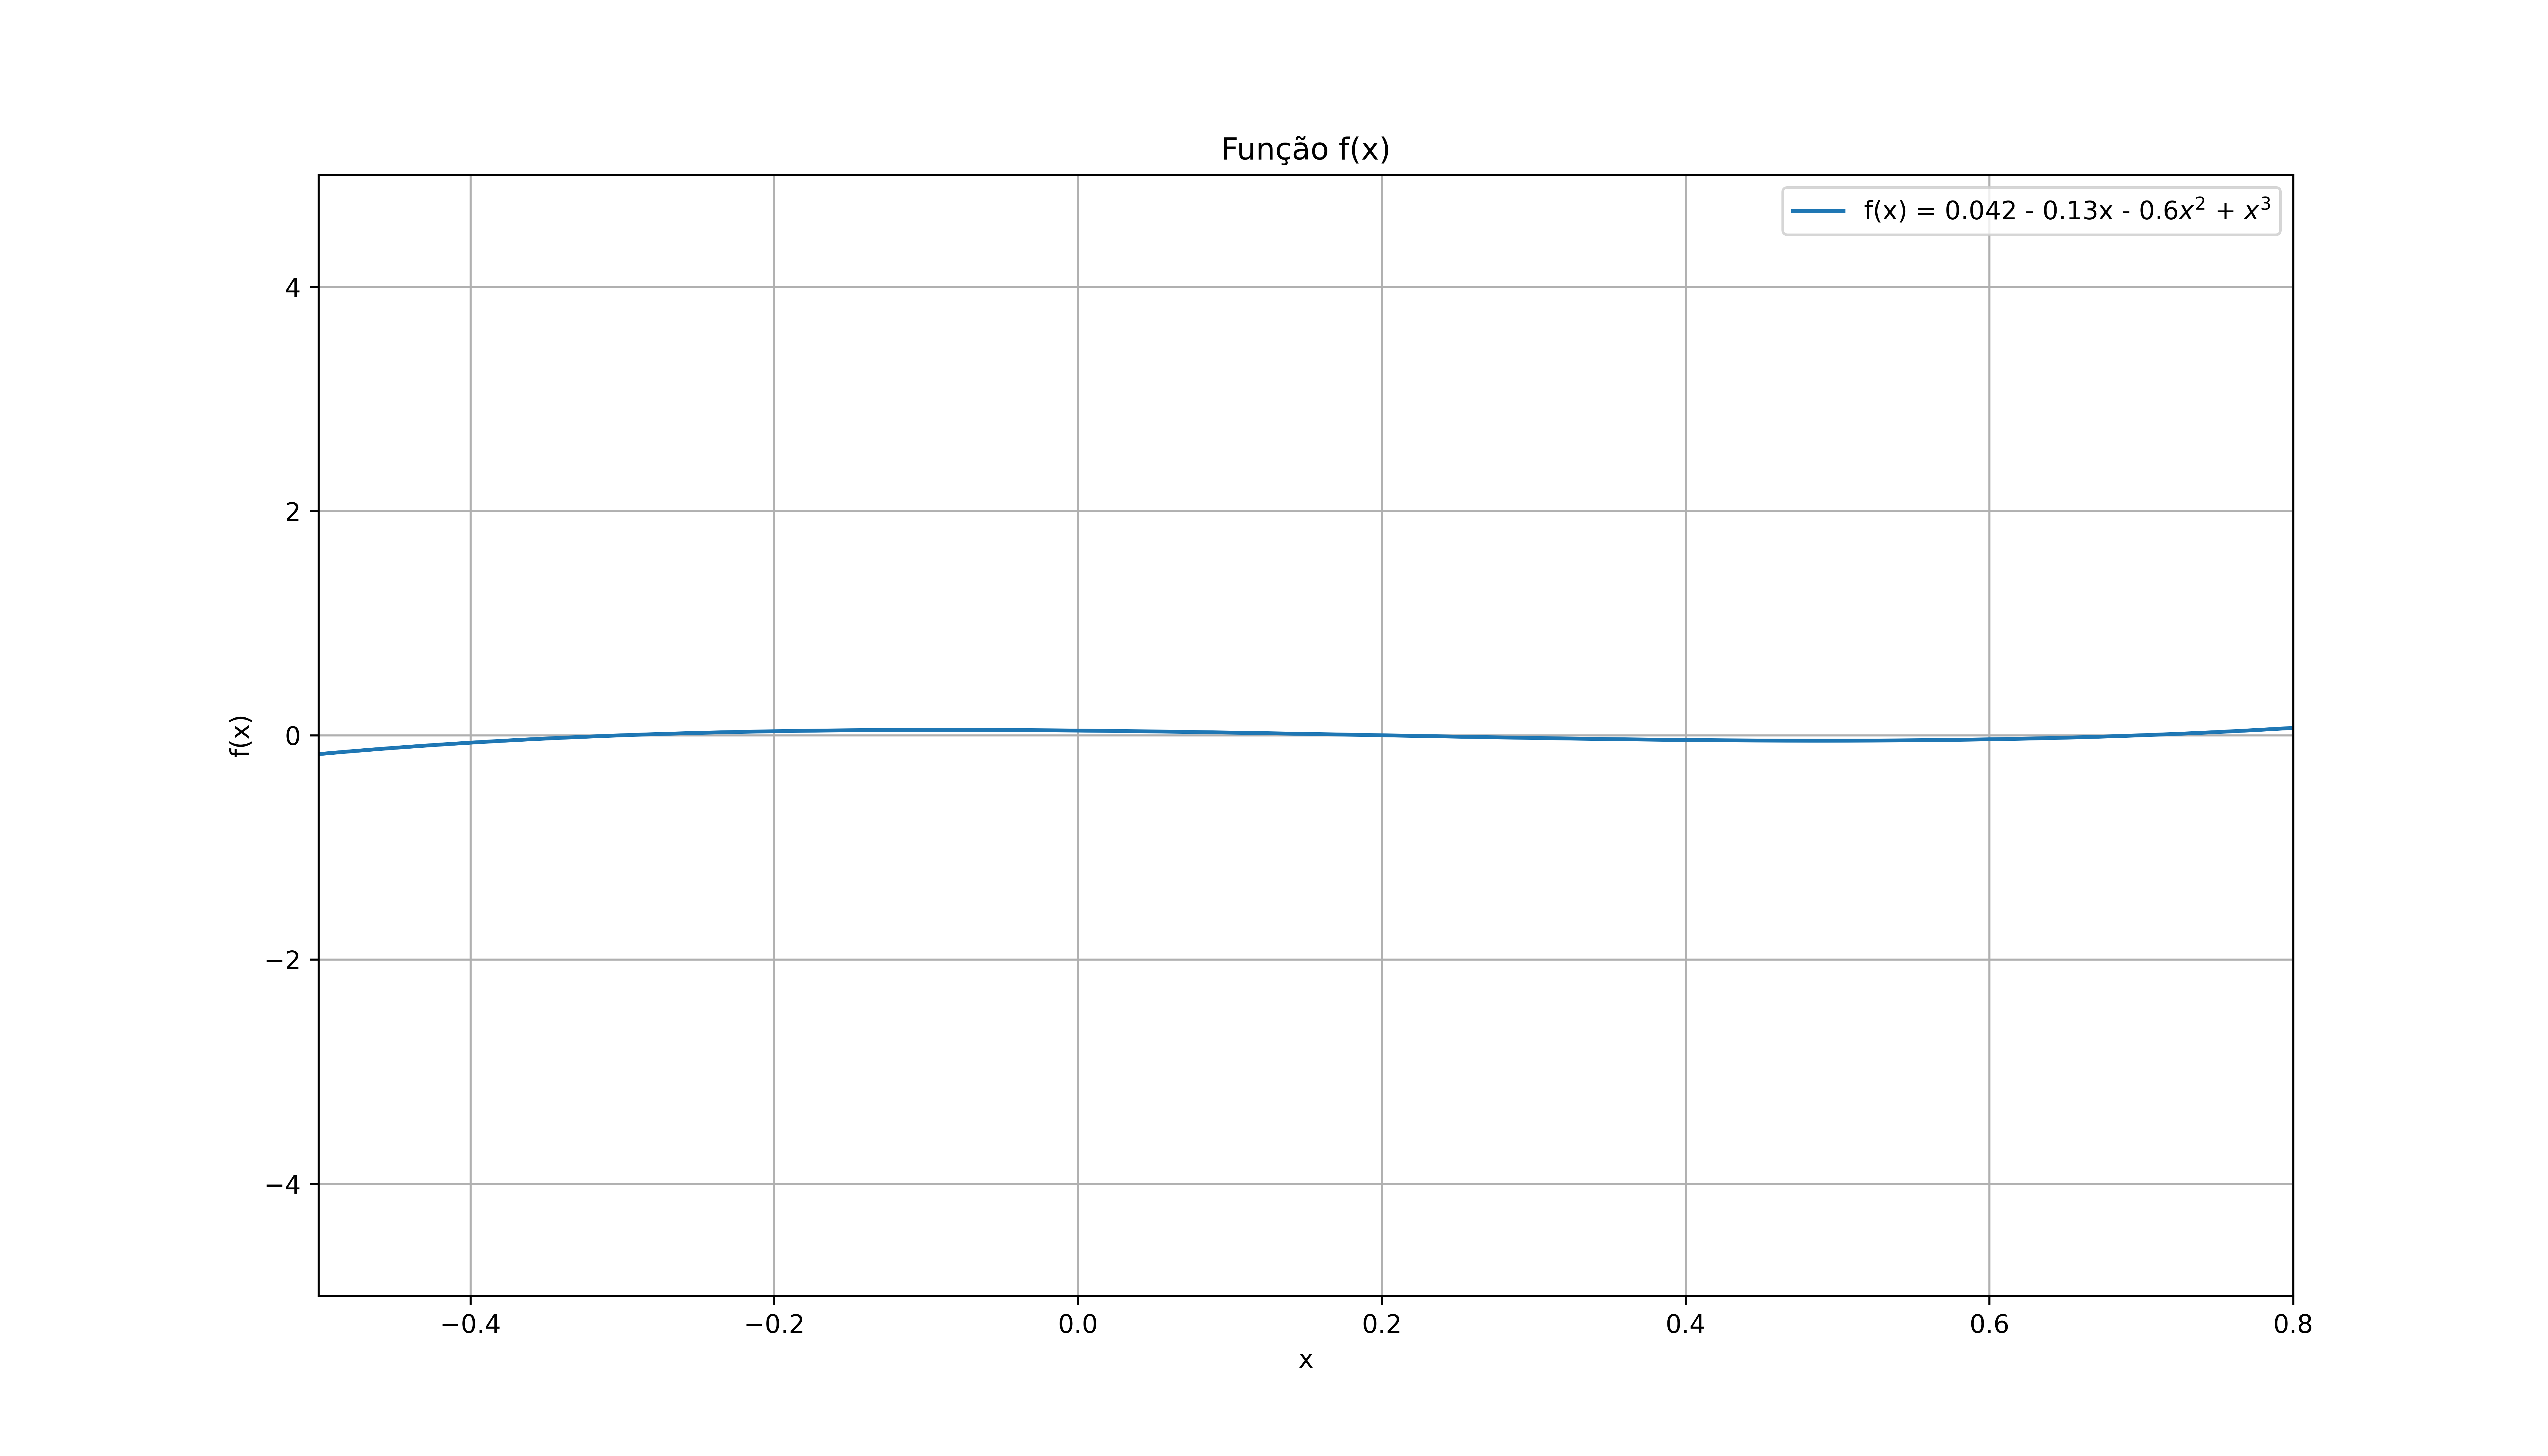
\includegraphics[width=16cm]{images/tarefa-3/tarefa-3-graf-2.png}
\caption*{Fonte: Compilado pelo Autor.}
\label{fig:tarefa 3 - Gráfico 2}
\end{figure}

\begin{figure}[H]
\centering
\caption{Gráfico da função $f$.}
\centering
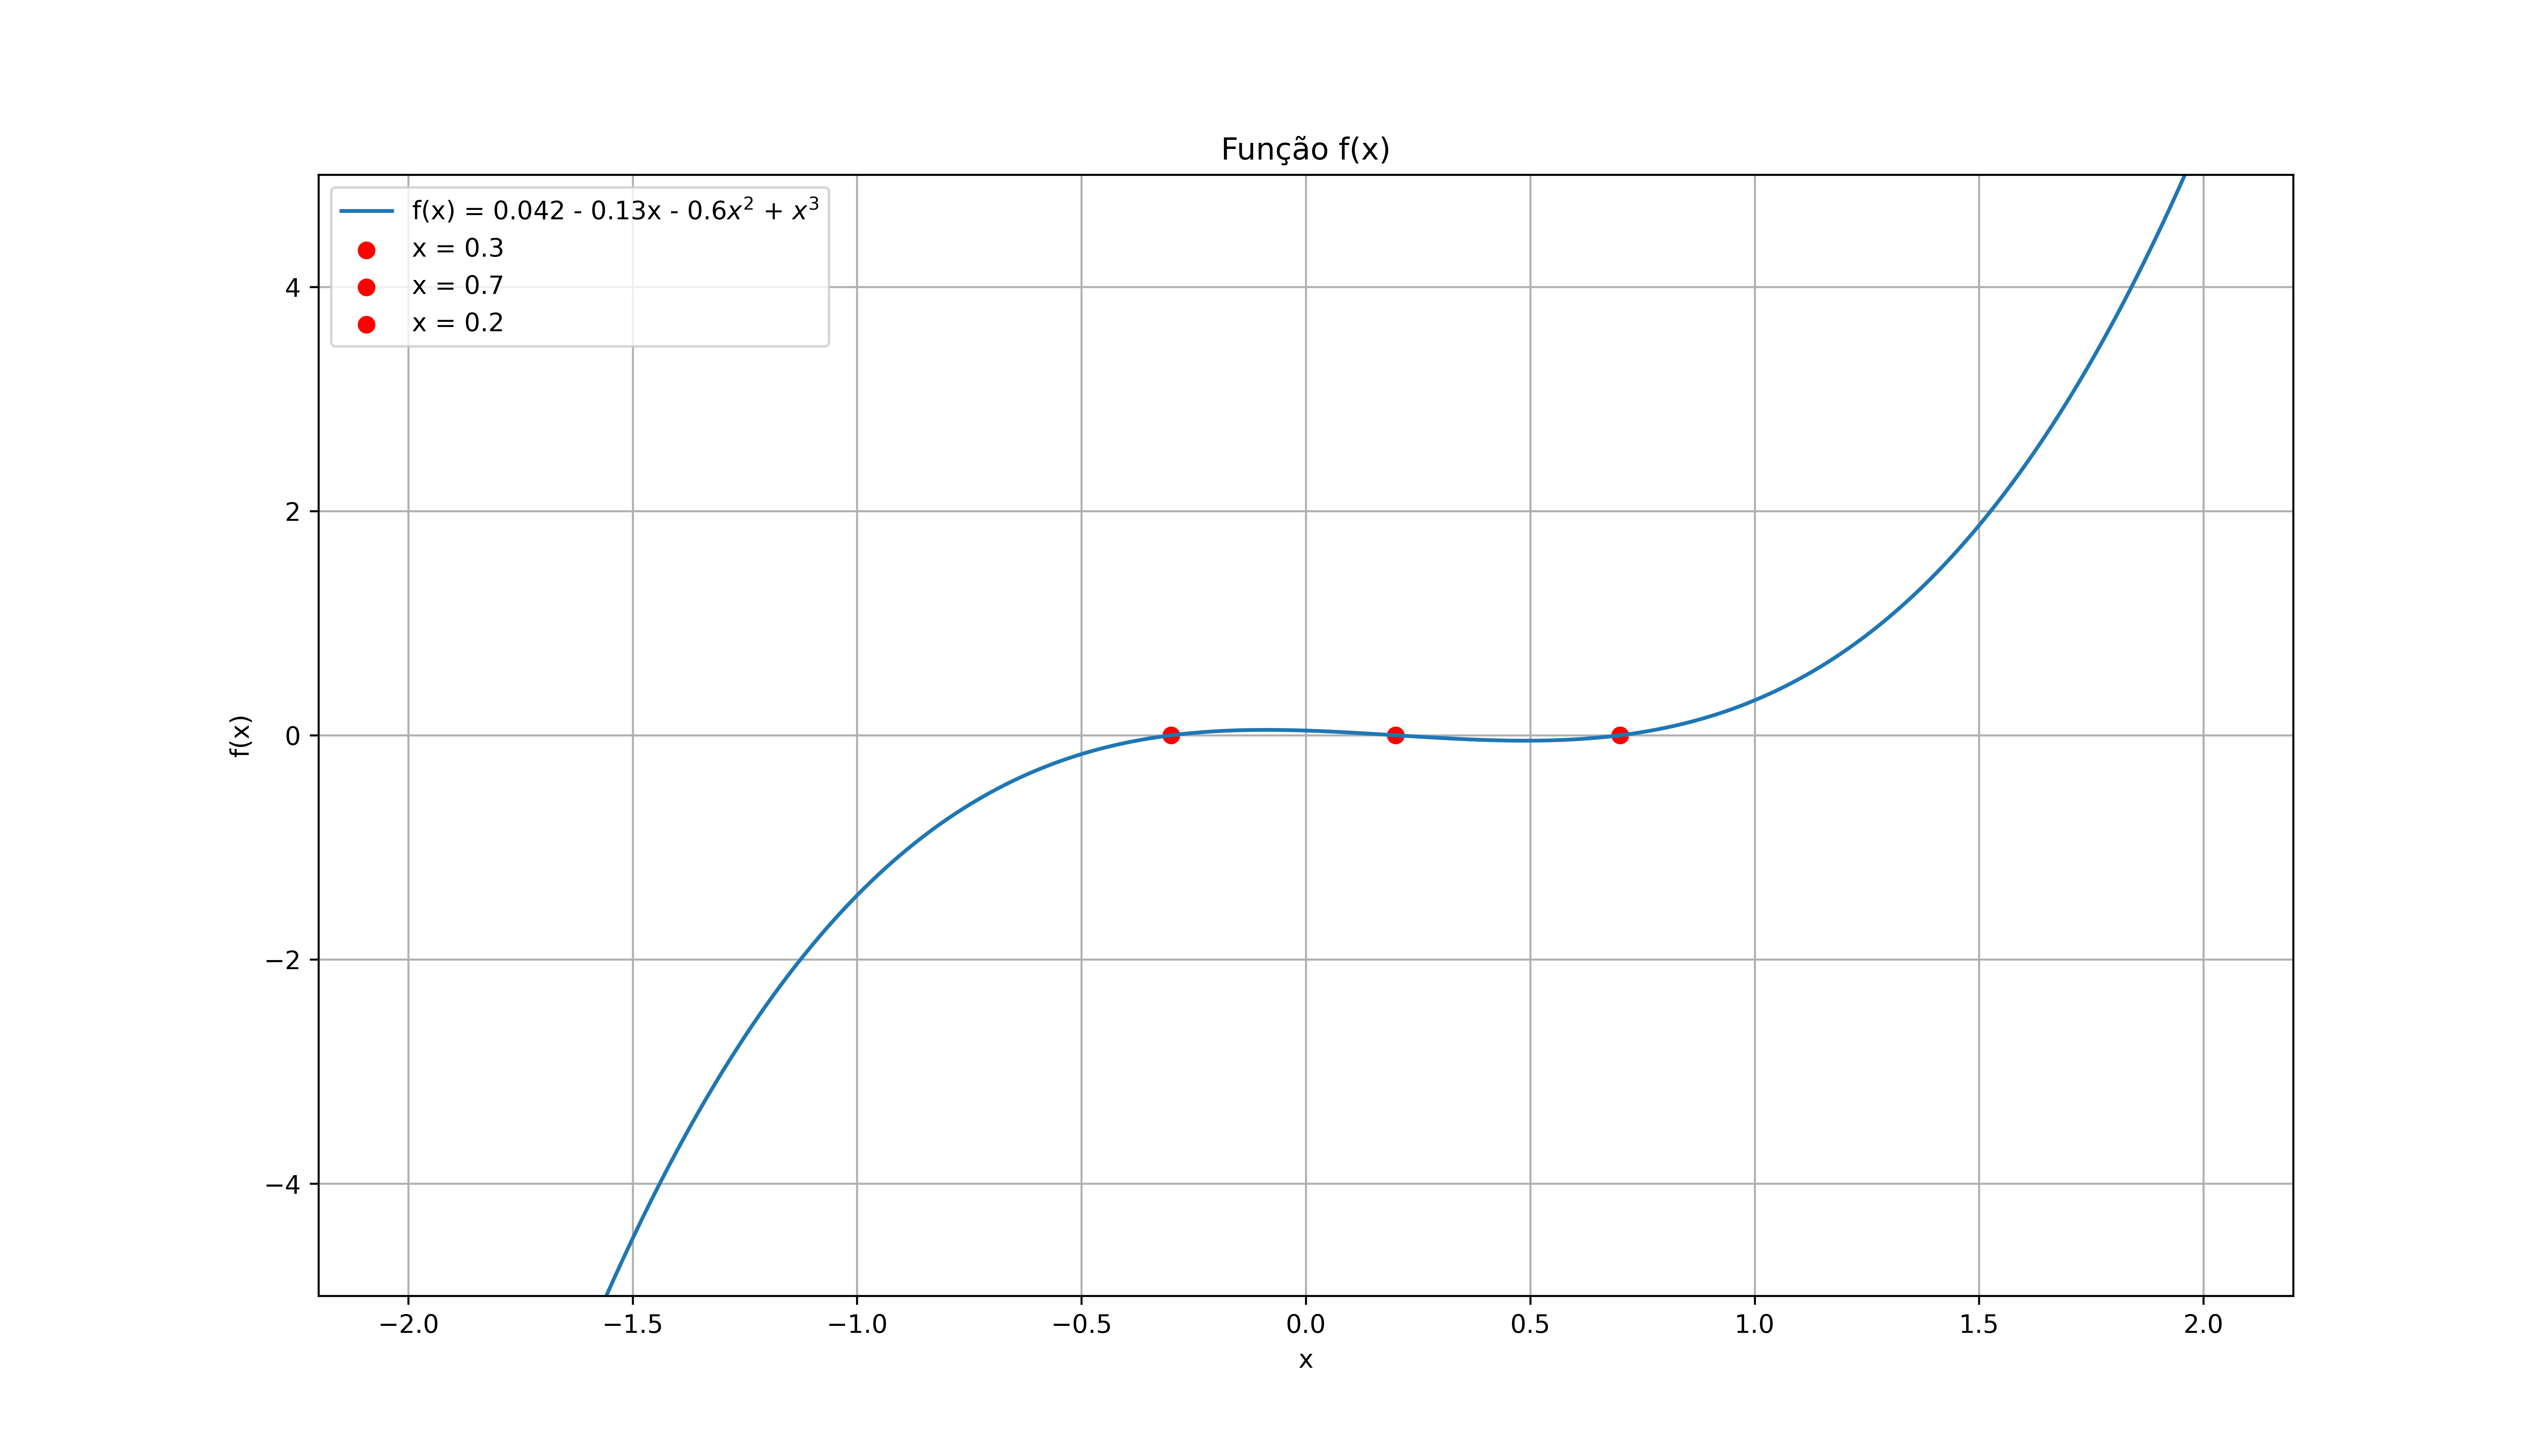
\includegraphics[width=16cm]{images/tarefa-3/tarefa-3-graf-3.png}
\caption*{Fonte: Compilado pelo Autor.}
\label{fig:tarefa 3 - Gráfico 3}
\end{figure}

\begin{figure}[H]
\centering
\caption{Gráfico da função $f$.}
\centering
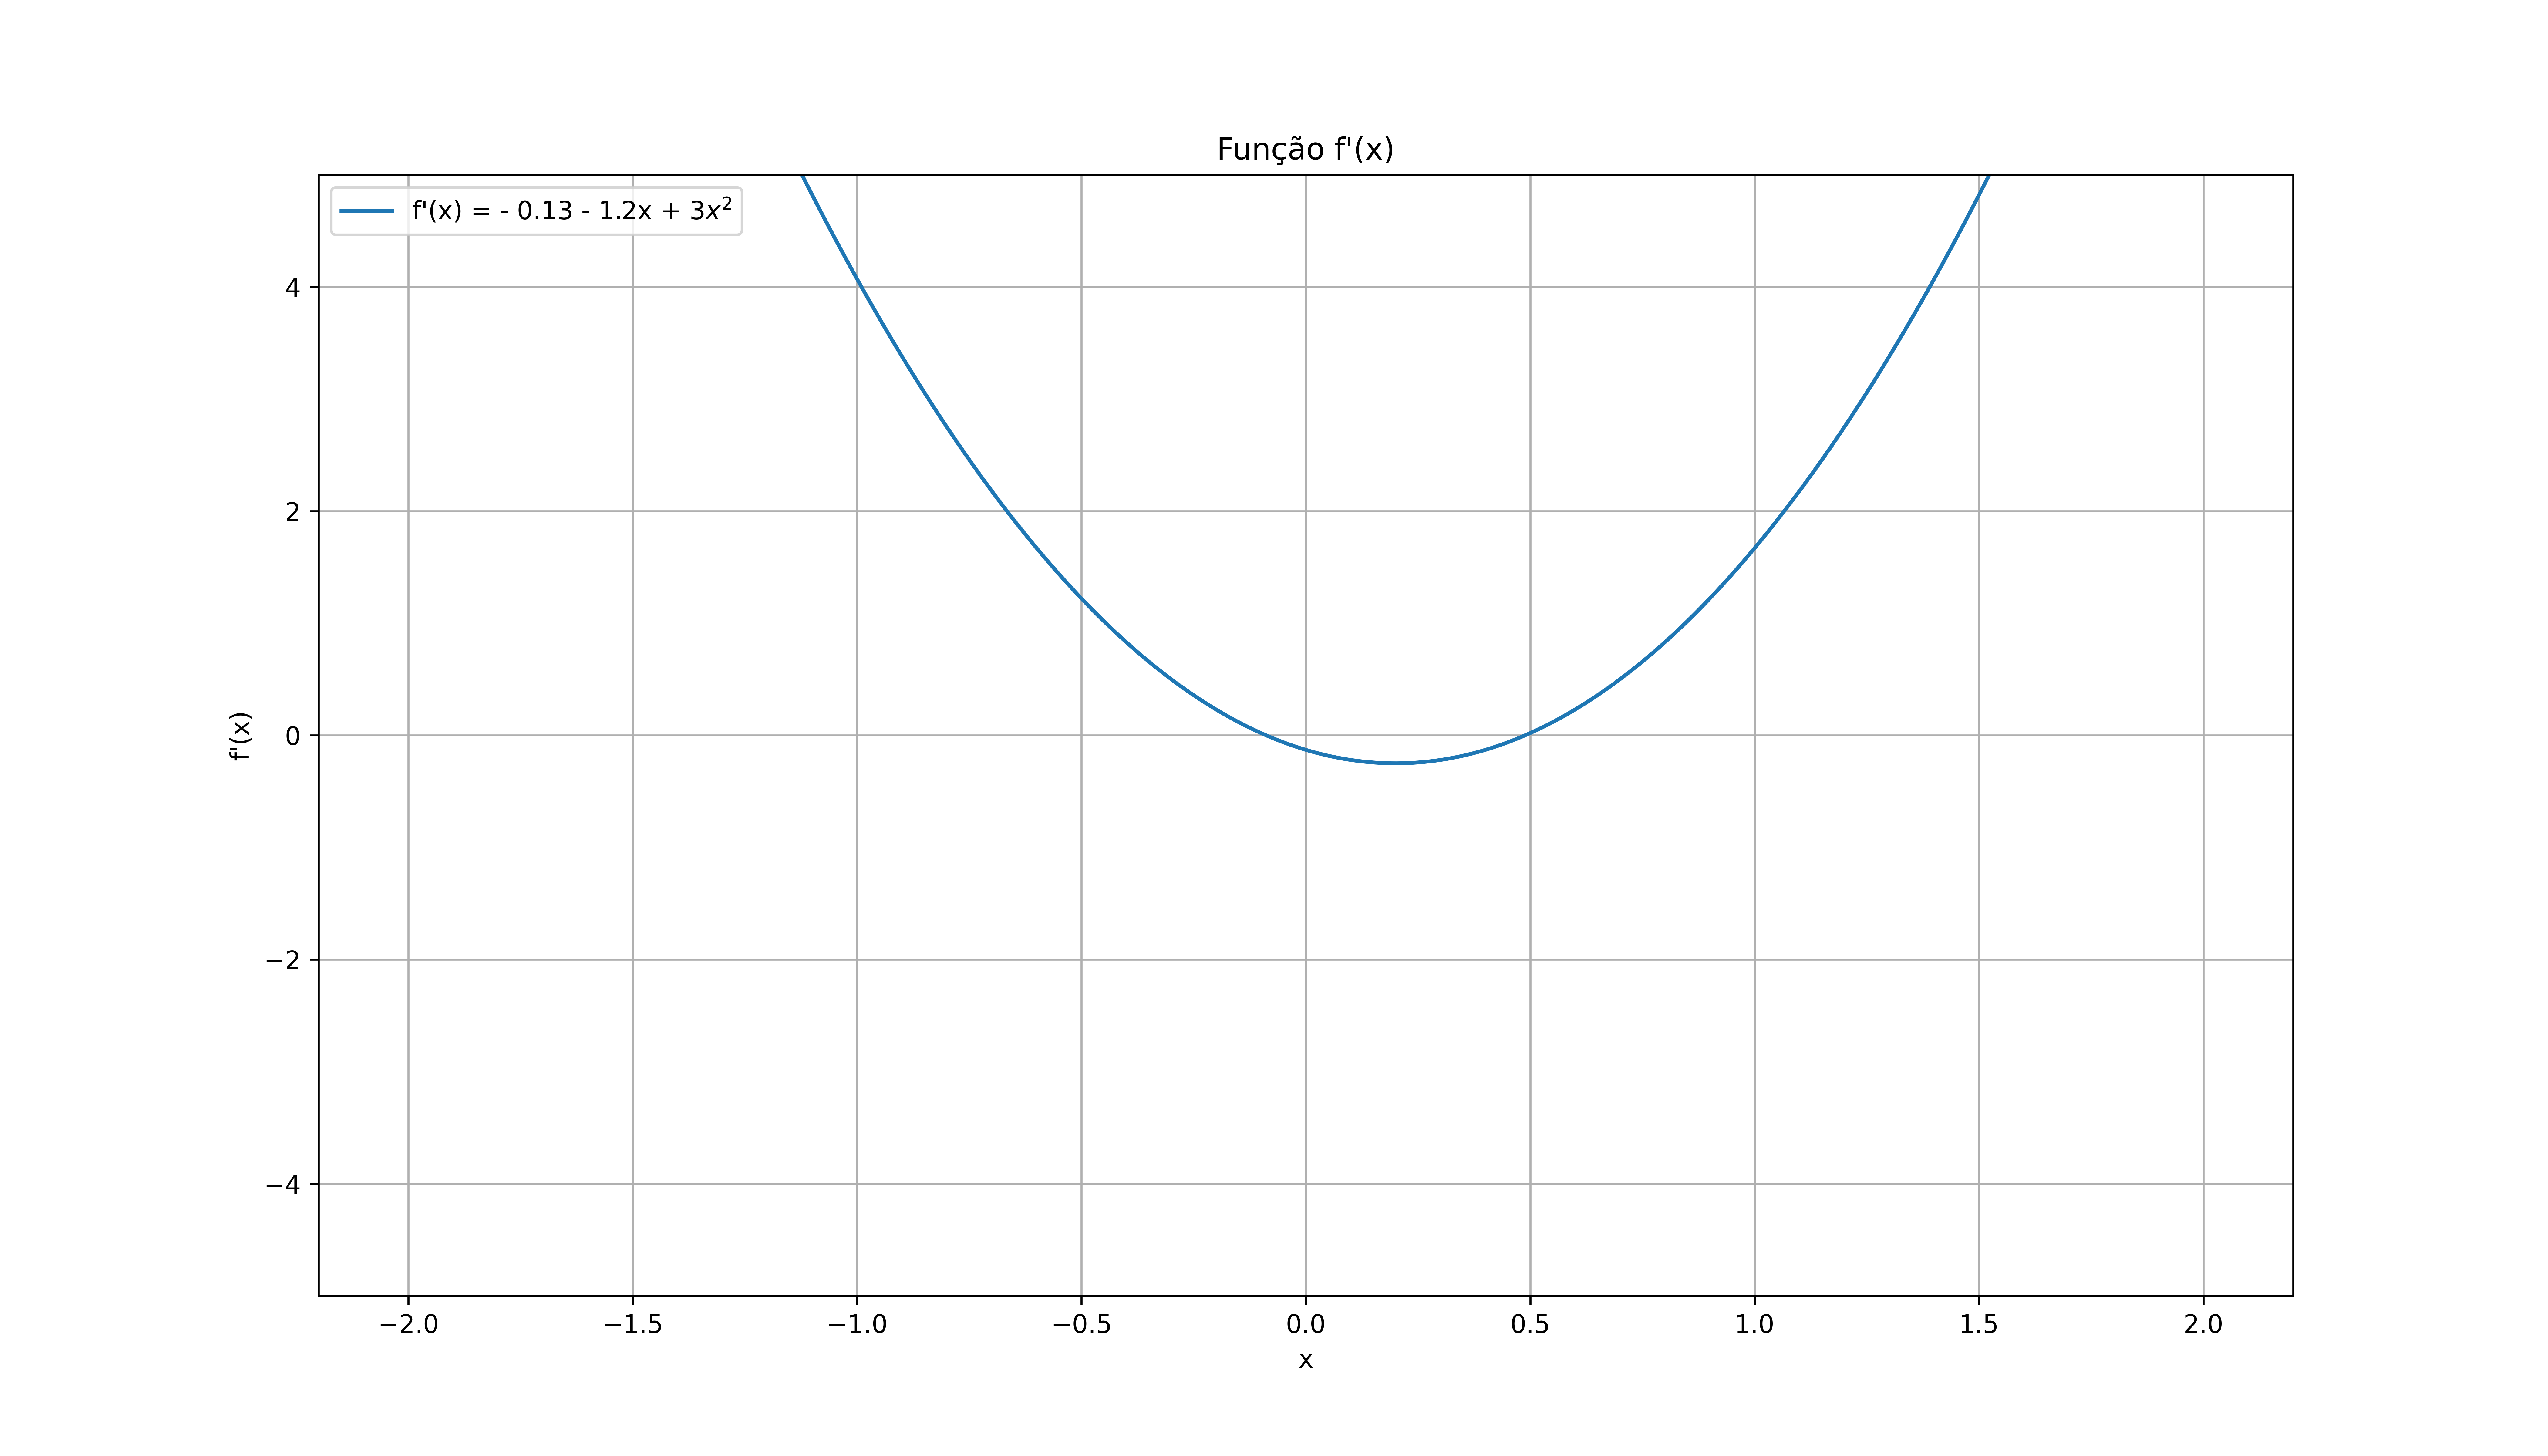
\includegraphics[width=16cm]{images/tarefa-3/tarefa-3-graf-4.png}
\caption*{Fonte: Compilado pelo Autor.}
\label{fig:tarefa 3 - Gráfico 4}
\end{figure}

\noindent
Ademais, é visto nos terminais os seguintes valores.

\begin{figure}[H]
\centering
\caption{Terminal a=-5.}
\centering
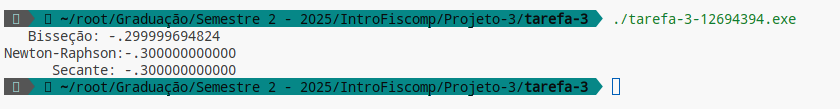
\includegraphics[width=16cm]{images/tarefa-3/tarefa-3-terminal-1.png}
\caption*{Fonte: Compilado pelo Autor.}
\label{fig:tarefa 3 - Terminal 1}
\end{figure}

\begin{figure}[H]
\centering
\caption{Terminal a=0.}
\centering
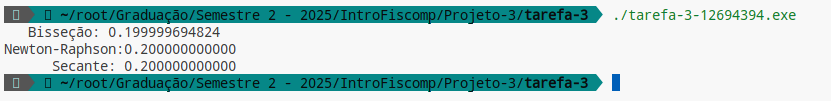
\includegraphics[width=16cm]{images/tarefa-3/tarefa-3-terminal-2.png}
\caption*{Fonte: Compilado pelo Autor.}
\label{fig:tarefa 3 - Terminal 2}
\end{figure}

\begin{figure}[H]
\centering
\caption{Terminal a=0.50.}
\centering
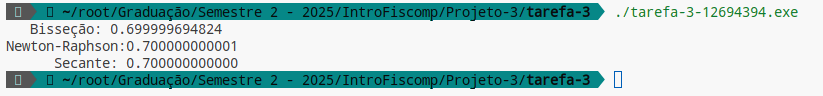
\includegraphics[width=16cm]{images/tarefa-3/tarefa-3-terminal-3.png}
\caption*{Fonte: Compilado pelo Autor.}
\label{fig:tarefa 3 - Terminal 3}
\end{figure}
